\documentclass[../../../../main.tex]{subfiles}
\begin{document}

半径1の円 $O$ の周を6等分する点を図のように順次 $A_1,A_2,\cdots,A_6$ とする．

弧 $A_2A_1A_6$ および半径 $OA_2$，$OA_6$ に接する円の中心を $P$ とし，
この円 $P$ の周と線分 $OP$ の交点を $B$ とする．
線分 $OA_3$ 上に $OQ=PA_1$ をみたすように点 $Q$ を定める．
$Q$ を中心とし $QA_3$ を半径とする円周と円 $P$ の交点のうちで，
直径 $A_1B$ に関し点 $A_2$ と同じ側にあるものを $C$ とする．

このとき四辺形 $OPCQ$ は平行四辺形であることを証明せよ．
また弧 $A_1A_2A_3$，弧 $A_3C$，弧 $CBA_1$ によって囲まれた領域(図の太線で囲まれた部分)の面積を求めよ．

\begin{figure}[htbp]
  \centering
  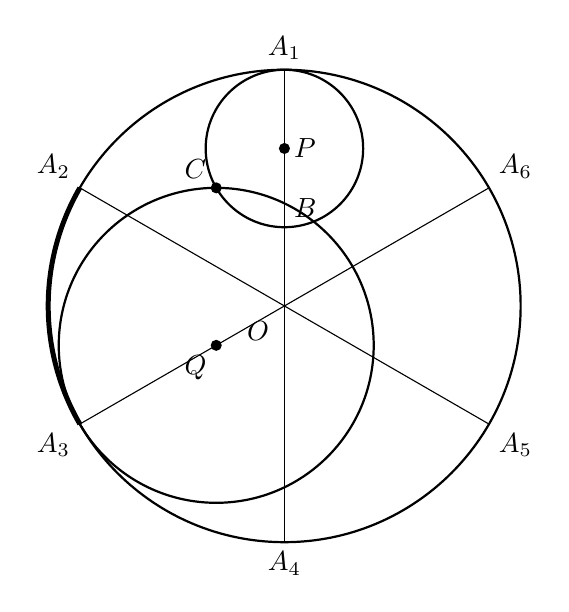
\begin{tikzpicture}[scale=2, >=stealth]
    \coordinate (O) at (0,0);
    \draw[thick] (O) circle (1.5);
    \node[below left=2pt] at (O) {$O$};

    \foreach \i/\ang in {1/90, 2/150, 3/210, 4/270, 5/330, 6/30} {
      \coordinate (A\i) at (\ang:1.5);
      \draw[thin] (O) -- (A\i);
    }

    \coordinate (P) at (0, 1.0);
    \draw[thick] (P) circle (0.5);
    \fill (P) circle (1pt) node[right] {$P$};

    \coordinate (B) at (0, 0.5);
    \node[above right] at (B) {$B$};

    \coordinate (Q) at (210:0.5);
    \fill (Q) circle (1pt) node[below left] {$Q$};
    \draw[thick] (Q) circle (1.0);

    \coordinate (C) at (-0.433, 0.75);
    \fill (C) circle (1pt) node[above left] {$C$};

    \draw[line width=1.8pt] (150:1.5) arc (150:210:1.5);

    \node[above] at (A1) {$A_1$};
    \node[above left] at (A2) {$A_2$};
    \node[below left] at (A3) {$A_3$};
    \node[below] at (A4) {$A_4$};
    \node[below right] at (A5) {$A_5$};
    \node[above right] at (A6) {$A_6$};
  \end{tikzpicture}
\end{figure}

\end{document}
